% f2015tjw_q06_circle.tex —— 2015 天津文科卷 Q6 圆与割线图（源 p1 栏 2）
%
% 源：.work/phase3-b10/source/2015天津文.pdf（p1 印 987）；实测清单 figure-inventory.md §F02
% 坐标换算：x_pic = x_pt − 535.0 ；y_pic = 200.0 − y_pt
%   （源页 pt、原点左上、y 向下；画布 x' 0.05–119.8、y' 12.5–139.9，单位 pt）
% 线宽：0.398 pt（源 `0.398 w` 实测）；无箭头、无虚线（p1 全页 `[] 0 d`）。
% 几何：圆心 O=(60.122, 76.348)，R=53.892；弦 AB 水平 y'=59.339；
%   三等分点 M=(43.056, 59.339)、N=(77.188, 59.339)（由 A 端按 1/3、2/3 内插）；
%   两割线共点 C=(42.262, 25.490)，另端 D=(49.747, 129.247)、E=(111.320, 93.357)。
%   三点落圆校验（清单实测）：C 半径 53.904、D 53.907、E 53.949（R=53.892，偏差 ≤0.06 pt）。
% 存疑照源复刻：§S-4 圆心「•」在源中是**文字字形**而非矢量圆点 —— 故本文件同样以文字绘制，
%   按源字形盒左上角 (58.55, 80.93) 定位，不用 \fill circle。
%   另：C 标签落在圆轮廓外、A/B 标签在弦端点外侧，均按源字形盒原样定位。
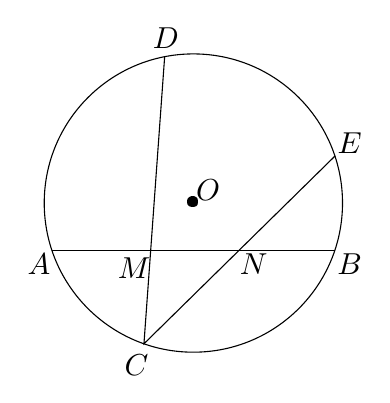
\begin{tikzpicture}[x=1pt, y=1pt, line width=0.398pt, every node/.style={font=\fontsize{10.5pt}{12.6pt}\selectfont,inner sep=0pt}]

  % ---- 圆 ----
  \draw (60.122,76.348) circle [radius=53.892];

  % ---- 弦 AB（A、B 恰在圆上） ----
  \draw (8.924,59.339) -- (111.320,59.339);

  % ---- 两条割线 CD、CE（共用 C，一条折线） ----
  \draw (49.747,129.247) -- (42.262,25.490) -- (111.320,93.357);

  % ---- 圆心墨点（源为文字字形而非矢量圆点，§S-4；故此处同样以文字绘制） ----
  % 源墨迹实测：圆盘 2.28 pt 见方、面积 4.68 pt^2、质心 (595.030, 123.445)；字形盒左上 (593.55,119.07)
  % 本稿按源「墨迹质心」定位（anchor=center），与源字形盒定位的差 0.2 pt 量级；
  % 探针 600dpi 复测：本稿墨点面积 4.46 pt^2、质心距源质心 0.94 pt（同量级，登记备终检微调）
  \node[anchor=center,inner sep=0] at (60.030,76.555) {\textbullet};

  % ---- 标签（源 pdftotext -bbox 字形盒左上角；inner sep=0） ----
  \node[anchor=north west,inner sep=0] at (45.25,139.92) {$D$};
  \node[anchor=north west,inner sep=0] at (112.07,101.99) {$E$};
  \node[anchor=north west,inner sep=0] at (60.90, 84.98) {$O$};
  \node[anchor=north west,inner sep=0] at ( 0.05, 58.11) {$A$};
  \node[anchor=north west,inner sep=0] at (32.64, 56.70) {$M$};
  \node[anchor=north west,inner sep=0] at (76.76, 58.11) {$N$};
  \node[anchor=north west,inner sep=0] at (112.00,58.11) {$B$};
  \node[anchor=north west,inner sep=0] at (35.09, 21.83) {$C$};

\end{tikzpicture}
